% Shared standalone design for the editable figure reconstructions.
\documentclass[tikz,border=5pt,10pt]{standalone}
\usepackage[T1]{fontenc}
\usepackage[utf8]{inputenc}
\usepackage{newpxtext,newpxmath}
\usepackage[scaled=.94]{sourcesanspro}
\usepackage{pgfplots}
\pgfplotsset{compat=1.18}
\usetikzlibrary{arrows.meta,calc,positioning,decorations.pathreplacing,
  decorations.markings,patterns,matrix,shapes.geometric,fit,backgrounds,
  intersections,angles,quotes}
\definecolor{ink}{HTML}{203746}
\definecolor{accent}{HTML}{146C78}
\definecolor{muted}{HTML}{667780}
\definecolor{signalred}{HTML}{B94B44}
\color{ink}
\tikzset{>=Latex,line width=.8pt,
  every node/.style={font=\small},
  axis/.style={->,draw=muted,line width=.5pt},
  guide/.style={draw=muted,dashed,line width=.45pt},
  curve/.style={draw=accent,line width=1pt},
  marker/.style={circle,fill=accent,inner sep=1.5pt},
  labelbox/.style={fill=white,inner sep=2pt}}

\begin{document}
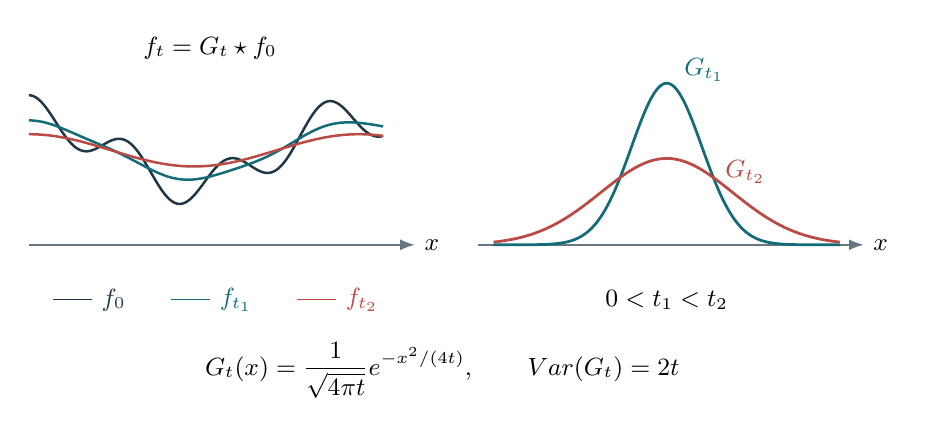
\begin{tikzpicture}[x=1cm,y=1cm]
\draw[axis] (0,0)--(4.9,0) node[right] {$x$};
\foreach \t/\col in {0/ink,.1/accent,.35/signalred} {
 \draw[draw=\col,line width=.9pt,domain=0:4.5,samples=201] plot (\x,{1.2+.45*exp(-2.25*\t)*cos(deg(1.5*\x))+.25*exp(-25*\t)*cos(deg(5*\x))});}
\node at (2.3,2.5) {$f_t=G_t\star f_0$};
\draw[ink] (.3,-.7)--(.8,-.7) node[right] {$f_0$};
\draw[accent] (1.8,-.7)--(2.3,-.7) node[right] {$f_{t_1}$};
\draw[signalred] (3.4,-.7)--(3.9,-.7) node[right] {$f_{t_2}$};
\begin{scope}[shift={(8.1,0)}]
\draw[axis] (-2.4,0)--(2.5,0) node[right] {$x$};
\draw[curve,domain=-2.2:2.2,samples=201] plot (\x,{2.3/sqrt(4*pi*.1)*exp(-\x*\x/(4*.1))});
\draw[signalred,line width=1pt,domain=-2.2:2.2,samples=201] plot (\x,{2.3/sqrt(4*pi*.35)*exp(-\x*\x/(4*.35))});
\node[accent,above right] at (.1,1.95) {$G_{t_1}$};\node[signalred,above] at (1,.65) {$G_{t_2}$};
\node at (0,-.7) {$0<t_1<t_2$};
\end{scope}
\node at (5.25,-1.6) {$\displaystyle G_t(x)=\frac{1}{\sqrt{4\pi t}}e^{-x^2/(4t)},\qquad \operatorname{Var}(G_t)=2t$};
\end{tikzpicture}
\end{document}
